\documentclass[12pt, a4paper]{article}

\usepackage[a4paper, margin=2.5cm]{geometry}
\usepackage{times}
\usepackage[T1]{fontenc}
\usepackage[utf8]{inputenc}
\usepackage{amsmath}
\usepackage{graphicx}
\usepackage{booktabs}
\usepackage{hyperref}
\usepackage{caption}
\usepackage{setspace}
\usepackage{titlesec}
\usepackage{xcolor}
\usepackage{parskip}
\usepackage{float}
\usepackage{enumitem}
\usepackage{fancyhdr}

% Spacing
\onehalfspacing

% Header/footer
\pagestyle{fancy}
\fancyhf{}
\lhead{\small Brain Tumor Segmentation Report}
\rhead{\small Musabek Musaev}
\cfoot{\thepage}
\renewcommand{\headrulewidth}{0.4pt}

% Section styling
\titleformat{\section}{\large\bfseries}{{\thesection.}}{0.5em}{}[\vspace{2pt}\hrule\vspace{4pt}]
\titleformat{\subsection}{\normalsize\bfseries}{\thesubsection.}{0.5em}{}

% Graphics path
\graphicspath{{paper_figures/}{results/}}

\begin{document}

% ── Title Page ────────────────────────────────────────────────────────────────
\begin{titlepage}
    \centering
    \vspace*{2cm}

    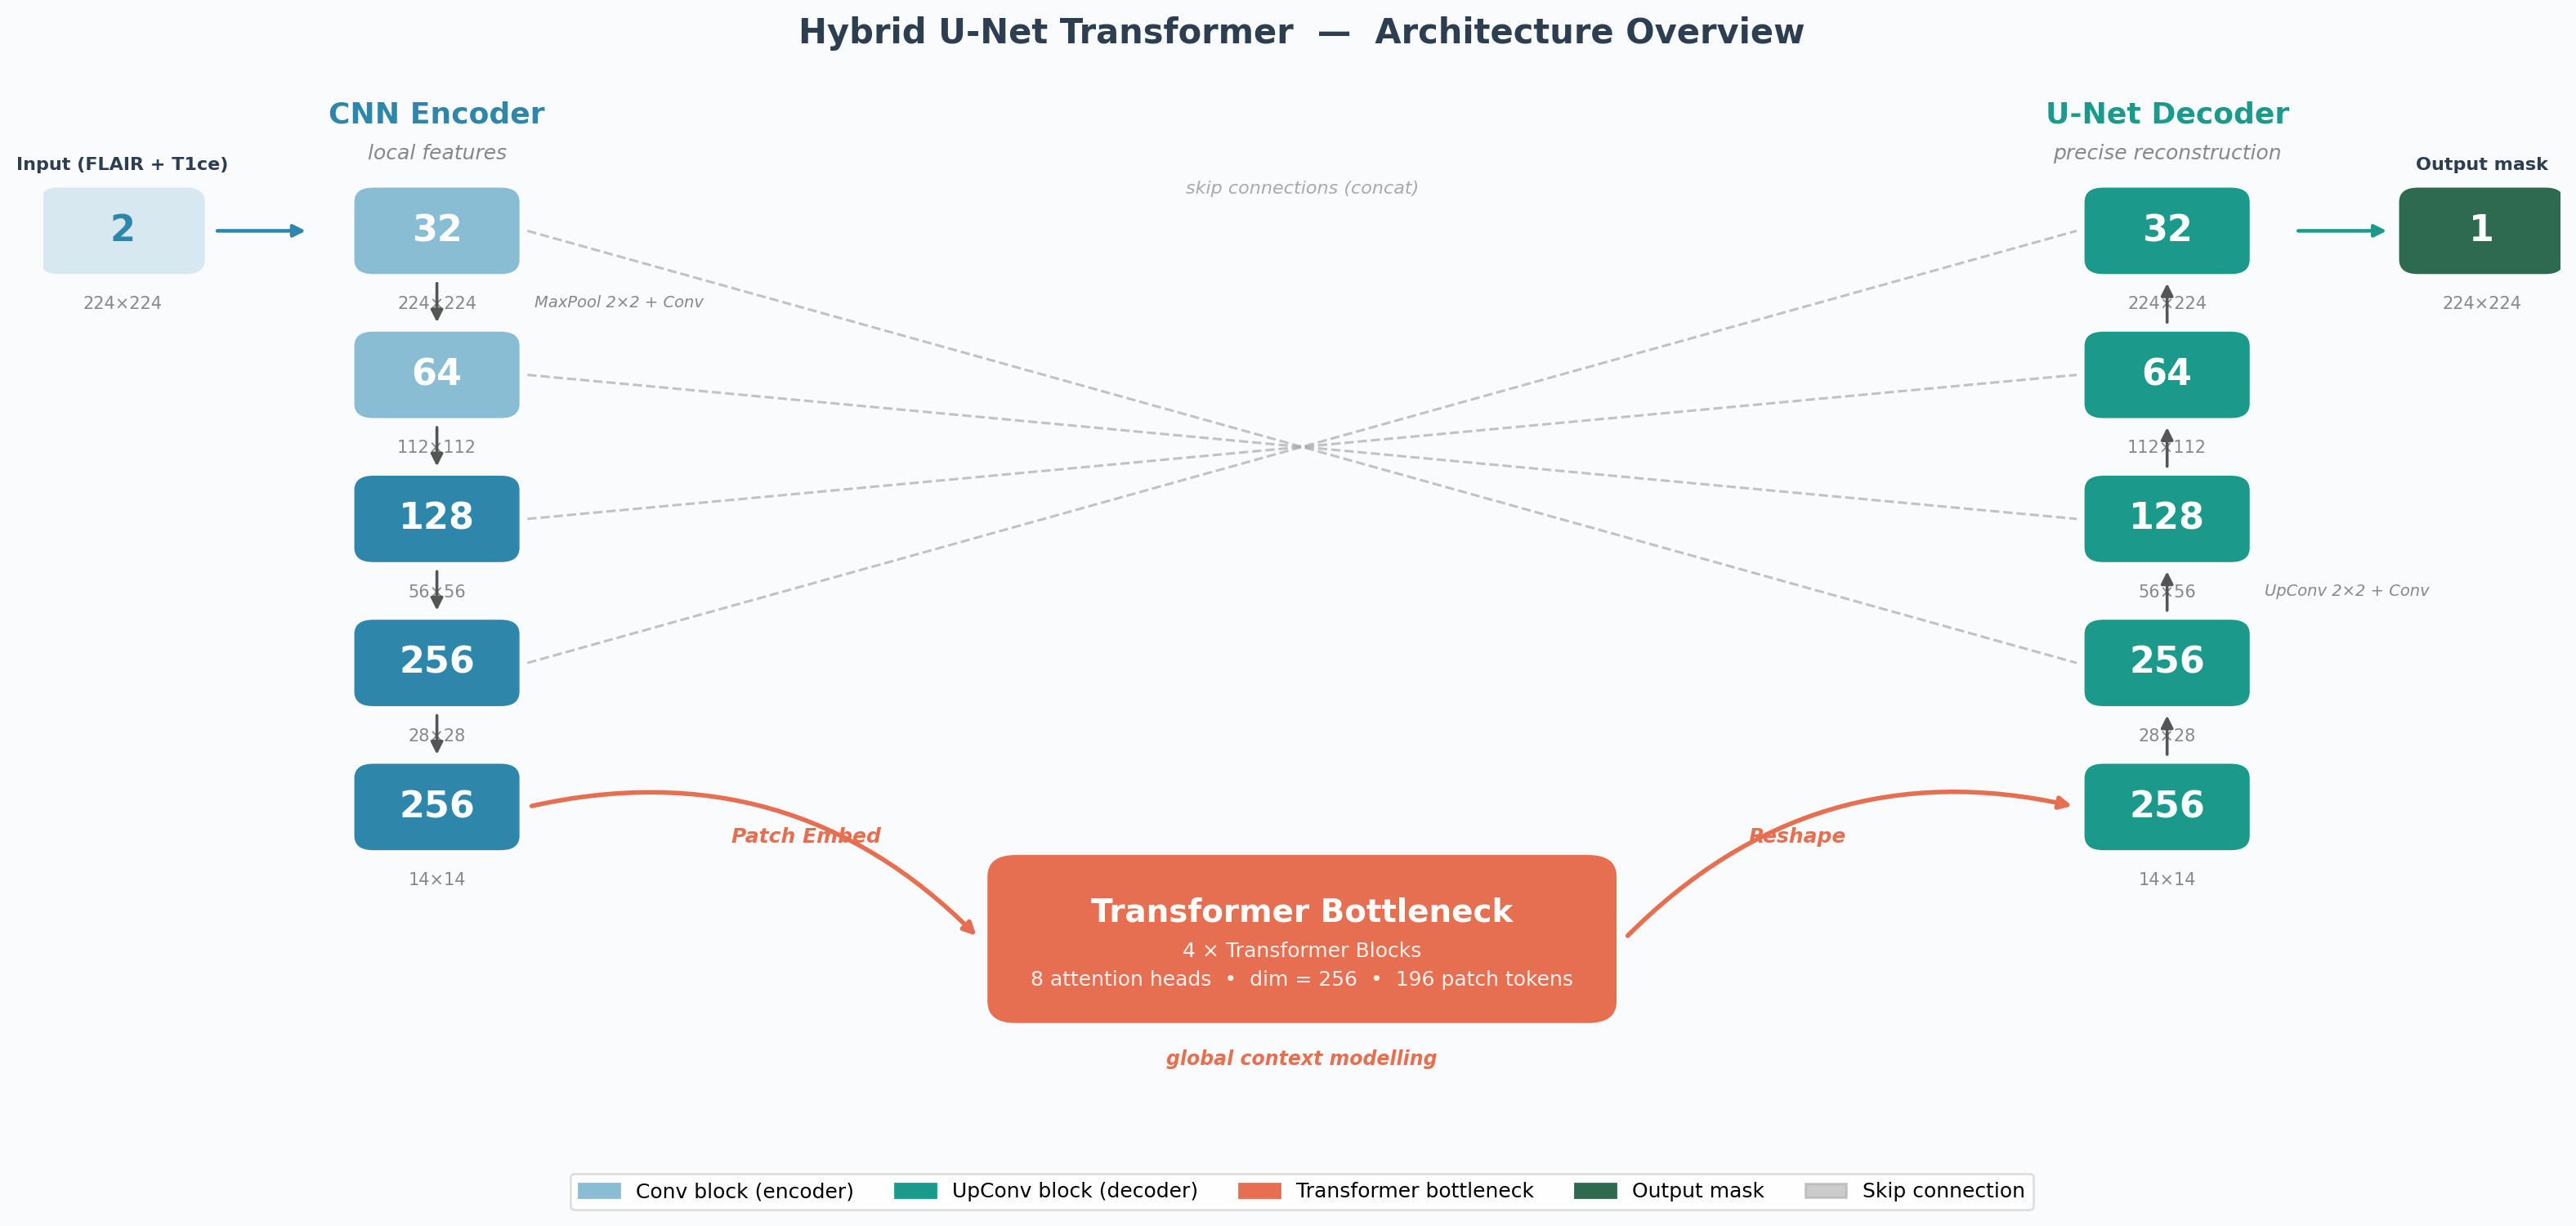
\includegraphics[width=0.55\textwidth]{fig1_architecture.png}

    \vspace{1.5cm}

    {\LARGE \textbf{Brain Tumor Segmentation Using\\[0.3em]
    Hybrid CNN-Transformer Architecture}}

    \vspace{1cm}

    {\large Research Report}

    \vspace{1.5cm}

    \begin{tabular}{rl}
        \textbf{Student:}  & Musabek Musaev \\[0.4em]
        \textbf{Course:}   & Research Seminar in HW/SW Aspects of \\
                           & Machine Learning for Smart Systems \\
                           & and Communications \\[0.4em]
        \textbf{Dataset:}  & BraTS 2020 \\[0.4em]
        \textbf{Hardware:} & NVIDIA RTX 4060 (8 GB VRAM) \\[0.4em]
        \textbf{Date:}     & May 2026 \\
    \end{tabular}

    \vfill

    \hrule
    \vspace{0.5cm}
    {\small This report presents the design, implementation, and evaluation of a
    hybrid deep learning model for automatic brain tumor segmentation from MRI scans.}

\end{titlepage}

% ── Table of Contents ─────────────────────────────────────────────────────────
\tableofcontents
\newpage

% ─────────────────────────────────────────────────────────────────────────────
\section{Introduction}
% ─────────────────────────────────────────────────────────────────────────────

Brain tumors are among the most dangerous diseases affecting the human brain. To diagnose and treat them, doctors use MRI (Magnetic Resonance Imaging) scans. However, manually marking the tumor region on hundreds of MRI slices is very time-consuming and varies between doctors. Automated deep learning models can help solve this problem by quickly and consistently detecting tumor regions.

This project develops and compares two deep learning models for brain tumor segmentation:

\begin{itemize}
    \item \textbf{Baseline U-Net} — a standard and well-known architecture for medical image segmentation
    \item \textbf{Hybrid U-Net Transformer} — our proposed model that combines a CNN with a Transformer module for better global understanding of the image
\end{itemize}

The main challenges addressed in this project are:
\begin{enumerate}
    \item \textbf{Class imbalance} — tumor pixels are only 1--5\% of total image pixels
    \item \textbf{Limited annotated data} — medical datasets are small
    \item \textbf{Hardware constraints} — training on a consumer GPU (8 GB VRAM)
\end{enumerate}

% ─────────────────────────────────────────────────────────────────────────────
\section{Dataset}
% ─────────────────────────────────────────────────────────────────────────────

The \textbf{BraTS 2020} (Brain Tumor Segmentation Challenge 2020) dataset was used for all experiments.

\begin{table}[H]
    \centering
    \caption{BraTS 2020 dataset overview}
    \begin{tabular}{ll}
        \toprule
        \textbf{Property} & \textbf{Value} \\
        \midrule
        Total patients & 369 glioma cases \\
        MRI modalities available & T1, T1ce, T2, FLAIR \\
        Modalities used & FLAIR + T1ce (2 input channels) \\
        Segmentation type & Binary (whole tumor vs.\ background) \\
        Image volume size & 240 $\times$ 240 $\times$ 155 voxels \\
        Training patients & 295 (80\%) \\
        Validation patients & 74 (20\%) \\
        \bottomrule
    \end{tabular}
\end{table}

We use only two MRI modalities:
\begin{itemize}
    \item \textbf{FLAIR} — shows the full tumor region including surrounding edema
    \item \textbf{T1ce} — shows the active enhancing tumor core
\end{itemize}

The data is split at the \textbf{patient level} (not slice level) to prevent any data leakage between training and validation.

% ─────────────────────────────────────────────────────────────────────────────
\section{Data Preprocessing and Augmentation}
% ─────────────────────────────────────────────────────────────────────────────

\subsection{Preprocessing}

Since training a 3D model requires too much GPU memory, we convert each 3D MRI volume into 2D axial slices. The preprocessing steps are:

\begin{enumerate}
    \item Load FLAIR and T1ce volumes from NIfTI format (.nii.gz)
    \item \textbf{Z-score normalize} each volume: subtract mean and divide by standard deviation, computed only on brain voxels (non-zero pixels)
    \item Extract axial slices in range $z \in [50, 130]$ — outer slices are mostly empty
    \item Skip slices with fewer than 10 tumor pixels
    \item Center-crop each slice to \textbf{224 $\times$ 224 pixels}
    \item Save as \texttt{.npy} files (images and masks separately)
\end{enumerate}

This produces approximately 18,000--22,000 training slices and 4,500--5,500 validation slices.

\subsection{Data Augmentation}

To improve generalization and reduce overfitting, the following augmentations are applied during training (image and mask together):

\begin{table}[H]
    \centering
    \caption{Data augmentation pipeline}
    \begin{tabular}{lc}
        \toprule
        \textbf{Augmentation} & \textbf{Probability} \\
        \midrule
        Horizontal flip & 50\% \\
        Vertical flip & 50\% \\
        Random 90° rotation & 50\% \\
        Affine transform (scale, rotate $\pm15°$) & 50\% \\
        Elastic deformation & 20\% \\
        Gaussian noise & 20\% \\
        Brightness / contrast $\pm10\%$ & 30\% \\
        \bottomrule
    \end{tabular}
\end{table}

No augmentation is applied during validation.

% ─────────────────────────────────────────────────────────────────────────────
\section{Model Architectures}
% ─────────────────────────────────────────────────────────────────────────────

\subsection{Baseline: Standard U-Net}

U-Net \cite{ronneberger2015} is the most widely used architecture for medical image segmentation. It consists of a symmetric encoder-decoder structure with skip connections.

\begin{itemize}
    \item \textbf{Encoder:} 4 stages, each with two 3$\times$3 convolutions + MaxPooling. Channels grow: 32 $\to$ 64 $\to$ 128 $\to$ 256
    \item \textbf{Bottleneck:} 512 channels at 14$\times$14 spatial resolution
    \item \textbf{Decoder:} 4 upsampling stages using transposed convolutions + skip connections from encoder
    \item \textbf{Output:} 1$\times$1 convolution producing a binary segmentation mask
    \item \textbf{Total parameters:} 7.8 million
\end{itemize}

\subsection{Proposed: Hybrid U-Net Transformer}

Our proposed model replaces the CNN bottleneck with a Transformer module. This gives the model a global view of the entire image at once, helping it reason about tumor extent and shape.

Figure \ref{fig:arch} shows the full architecture.

\begin{figure}[H]
    \centering
    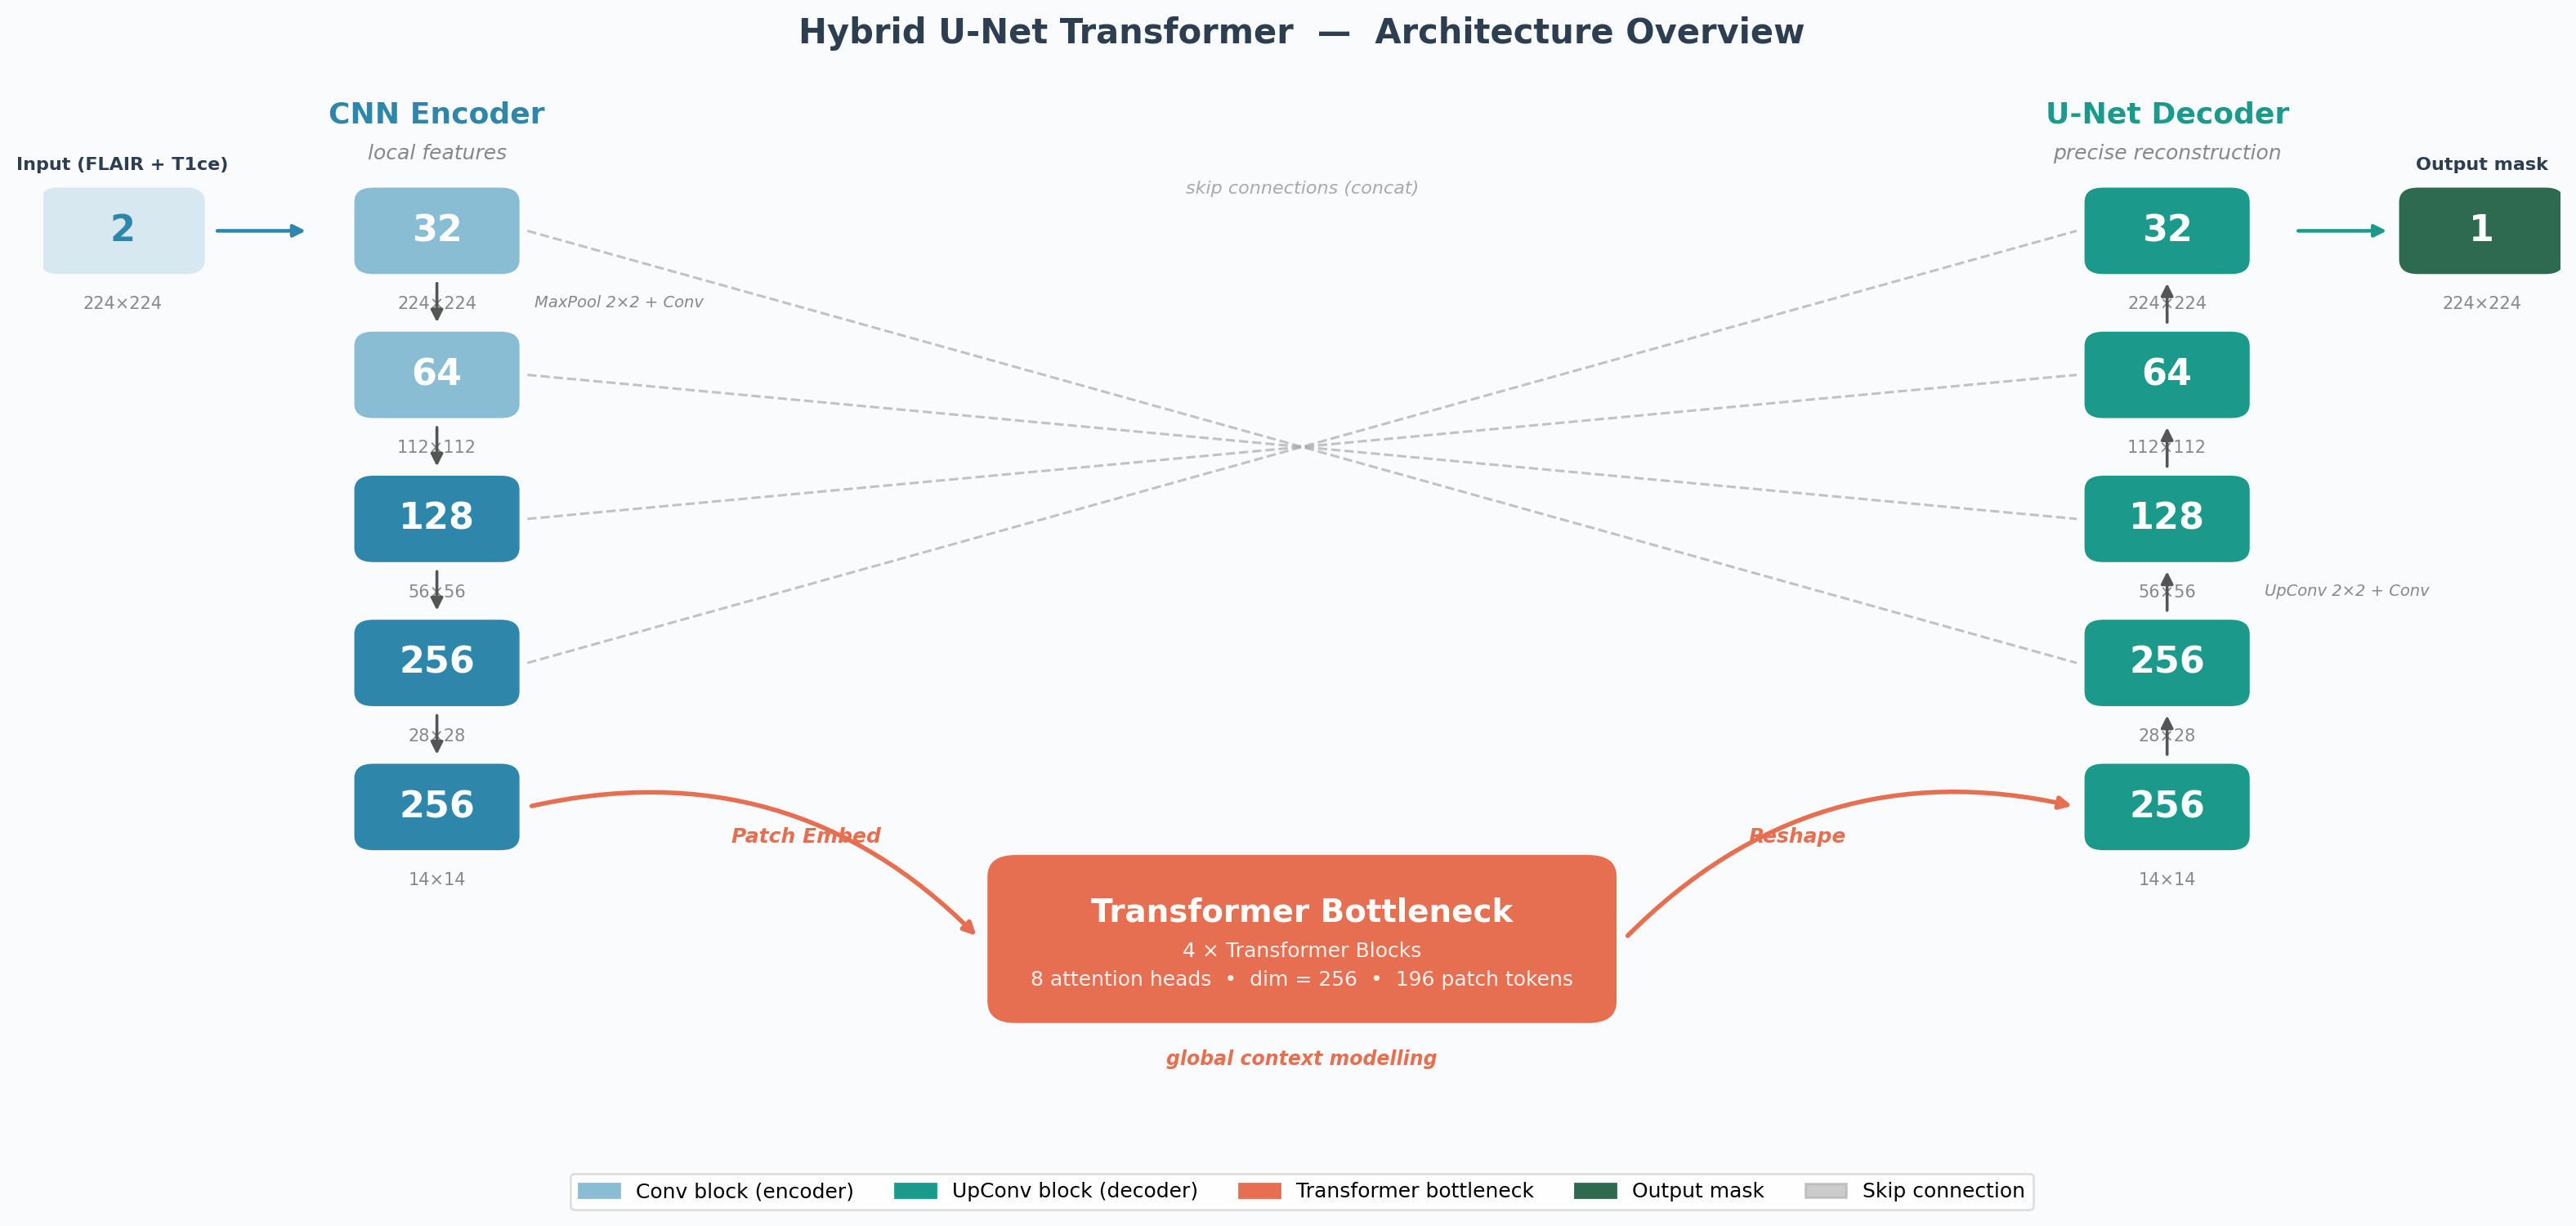
\includegraphics[width=\textwidth]{fig1_architecture.png}
    \caption{Hybrid U-Net Transformer architecture. Blue blocks: CNN encoder; purple: Transformer bottleneck; green blocks: CNN decoder; orange markers: deep supervision output heads; dashed arcs: skip connections.}
    \label{fig:arch}
\end{figure}

\textbf{Key components:}

\begin{itemize}
    \item \textbf{CNN Encoder:} Same as U-Net, 4 stages (32 $\to$ 64 $\to$ 128 $\to$ 256 channels)
    \item \textbf{Patch Embedding:} 1$\times$1 convolution projects 256 channels to Transformer dimension $d=256$. The 14$\times$14 spatial grid is flattened into 196 tokens
    \item \textbf{Positional Encoding:} Learnable position embeddings added to each token
    \item \textbf{Transformer:} 4 blocks, each with Multi-Head Self-Attention (8 heads) and Feed-Forward Network (expansion ratio 4, GELU activation, dropout 0.1)
    \item \textbf{CNN Decoder:} 4 upsampling blocks with skip connections
    \item \textbf{Deep Supervision:} Auxiliary prediction heads at 28$\times$28, 56$\times$56, and 112$\times$112 resolutions. These extra outputs help the model learn better during training by providing gradient signals to early layers
    \item \textbf{Total parameters:} 12.4 million
\end{itemize}

% ─────────────────────────────────────────────────────────────────────────────
\section{Loss Function}
% ─────────────────────────────────────────────────────────────────────────────

A combined loss function is used to handle class imbalance:

\begin{equation}
    \mathcal{L}_{total} = 0.7 \cdot \mathcal{L}_{Dice} + 0.3 \cdot \mathcal{L}_{Focal}
\end{equation}

\textbf{Dice Loss} \cite{milletari2016} directly optimizes the overlap between prediction and ground truth. It handles class imbalance naturally:

\begin{equation}
    \mathcal{L}_{Dice} = 1 - \frac{2\sum_i p_i y_i + 1}{\sum_i p_i + \sum_i y_i + 1}
\end{equation}

\textbf{Focal Loss} \cite{lin2017} forces the model to focus on hard examples (small tumors, boundary pixels) by down-weighting easy background pixels:

\begin{equation}
    \mathcal{L}_{Focal} = -\frac{1}{N} \sum_i \alpha_t (1 - p_t)^{\gamma} \cdot \text{BCE}(\hat{y}_i, y_i)
\end{equation}

where $\gamma = 2.0$ and $\alpha = 0.25$.

% ─────────────────────────────────────────────────────────────────────────────
\section{Training Setup}
% ─────────────────────────────────────────────────────────────────────────────

\begin{table}[H]
    \centering
    \caption{Training hyperparameters for both models}
    \begin{tabular}{lll}
        \toprule
        \textbf{Parameter} & \textbf{U-Net} & \textbf{Hybrid} \\
        \midrule
        Optimizer & AdamW & AdamW \\
        Learning rate & $1 \times 10^{-4}$ & $1 \times 10^{-4}$ \\
        Weight decay & $1 \times 10^{-5}$ & $1 \times 10^{-5}$ \\
        Batch size & 16 & 8 \\
        Max epochs & 50 & 50 \\
        LR schedule & Cosine Annealing & Cosine Annealing \\
        Warmup & 3 epochs & 3 epochs \\
        Early stopping & patience = 10 & patience = 10 \\
        Mixed precision & FP16 (AMP) & FP16 (AMP) \\
        Gradient clipping & max norm 1.0 & max norm 1.0 \\
        GPU & RTX 4060 8GB & RTX 4060 8GB \\
        Training time & $\sim$2--3 hours & $\sim$3--4 hours \\
        \bottomrule
    \end{tabular}
\end{table}

% ─────────────────────────────────────────────────────────────────────────────
\section{Evaluation Metrics}
% ─────────────────────────────────────────────────────────────────────────────

Three metrics are used to evaluate both models:

\begin{itemize}
    \item \textbf{Dice Similarity Coefficient (DSC):} Measures the overlap between prediction and ground truth. Range 0--1, higher is better.
    \begin{equation}
        DSC = \frac{2 |P \cap G|}{|P| + |G|}
    \end{equation}

    \item \textbf{Intersection over Union (IoU):} Similar to Dice but stricter. Range 0--1, higher is better.
    \begin{equation}
        IoU = \frac{|P \cap G|}{|P \cup G|}
    \end{equation}

    \item \textbf{Hausdorff Distance (HD):} Measures the worst-case boundary error in pixels. Lower is better. Important for clinical use.
\end{itemize}

% ─────────────────────────────────────────────────────────────────────────────
\section{Results}
% ─────────────────────────────────────────────────────────────────────────────

\subsection{Quantitative Results}

Both models were evaluated on \textbf{1,176 validation slices} from 74 patients.

\begin{table}[H]
    \centering
    \caption{Comparison of U-Net and Hybrid U-Net Transformer on BraTS 2020 validation set. $\uparrow$ = higher is better, $\downarrow$ = lower is better.}
    \begin{tabular}{lccccc}
        \toprule
        \textbf{Model} & \textbf{Mean Dice} $\uparrow$ & \textbf{Median Dice} $\uparrow$ & \textbf{Mean IoU} $\uparrow$ & \textbf{Mean HD (px)} $\downarrow$ & \textbf{Dice Std} $\downarrow$ \\
        \midrule
        Baseline U-Net       & 0.8339 & 0.9073 & 0.7512 & 14.984 & 0.1993 \\
        \textbf{Hybrid (ours)} & \textbf{0.8409} & \textbf{0.9081} & \textbf{0.7577} & \textbf{14.266} & \textbf{0.1853} \\
        \midrule
        Improvement & +0.0070 & +0.0008 & +0.0066 & $-$0.718 & $-$0.0140 \\
        \bottomrule
    \end{tabular}
\end{table}

\begin{figure}[H]
    \centering
    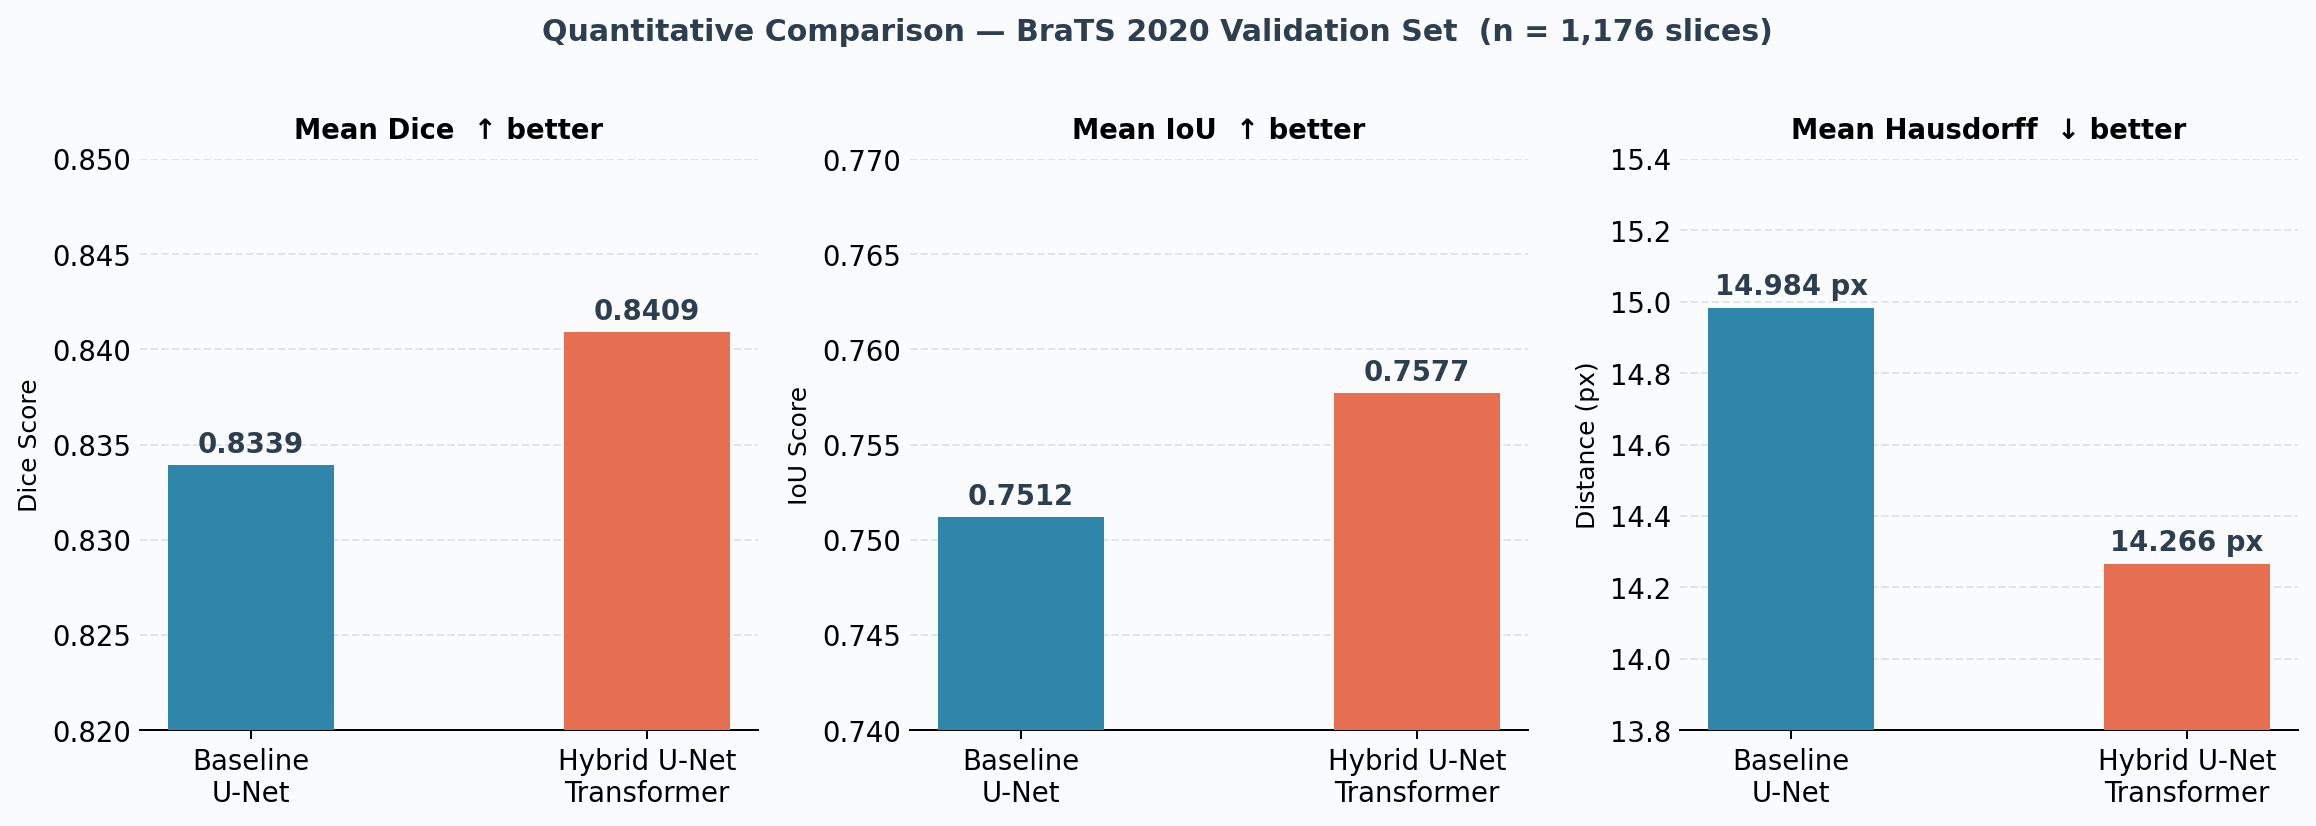
\includegraphics[width=\textwidth]{fig2_metrics.png}
    \caption{Mean Dice, IoU, and Hausdorff Distance comparison. The Hybrid model outperforms the baseline on all three metrics.}
\end{figure}

\subsection{Per-Slice Dice Distribution}

\begin{figure}[H]
    \centering
    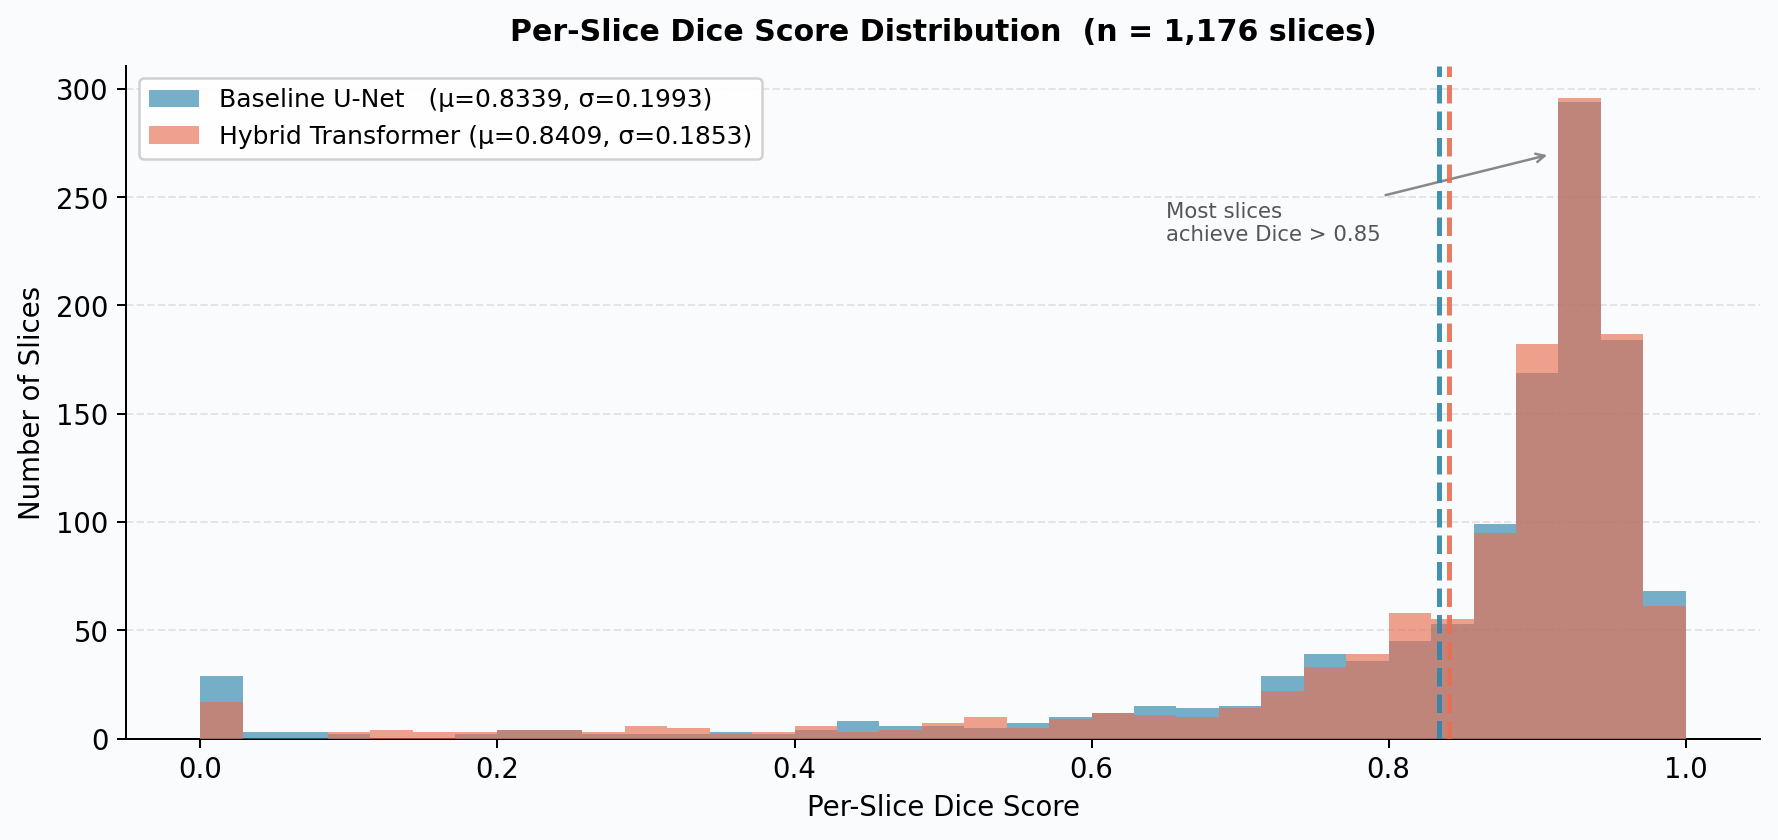
\includegraphics[width=0.85\textwidth]{fig3_distribution.png}
    \caption{Distribution of Dice scores across all 1,176 validation slices. The Hybrid model (orange) has fewer low-Dice outliers and a lower standard deviation (0.1853 vs.\ 0.1993).}
\end{figure}

The distribution is left-skewed for both models — most slices achieve high Dice ($>$0.85), but a small number of difficult slices (small or irregular tumors) pull the mean down. The Hybrid model handles these difficult cases more reliably.

\subsection{Visual Comparison}

\begin{figure}[H]
    \centering
    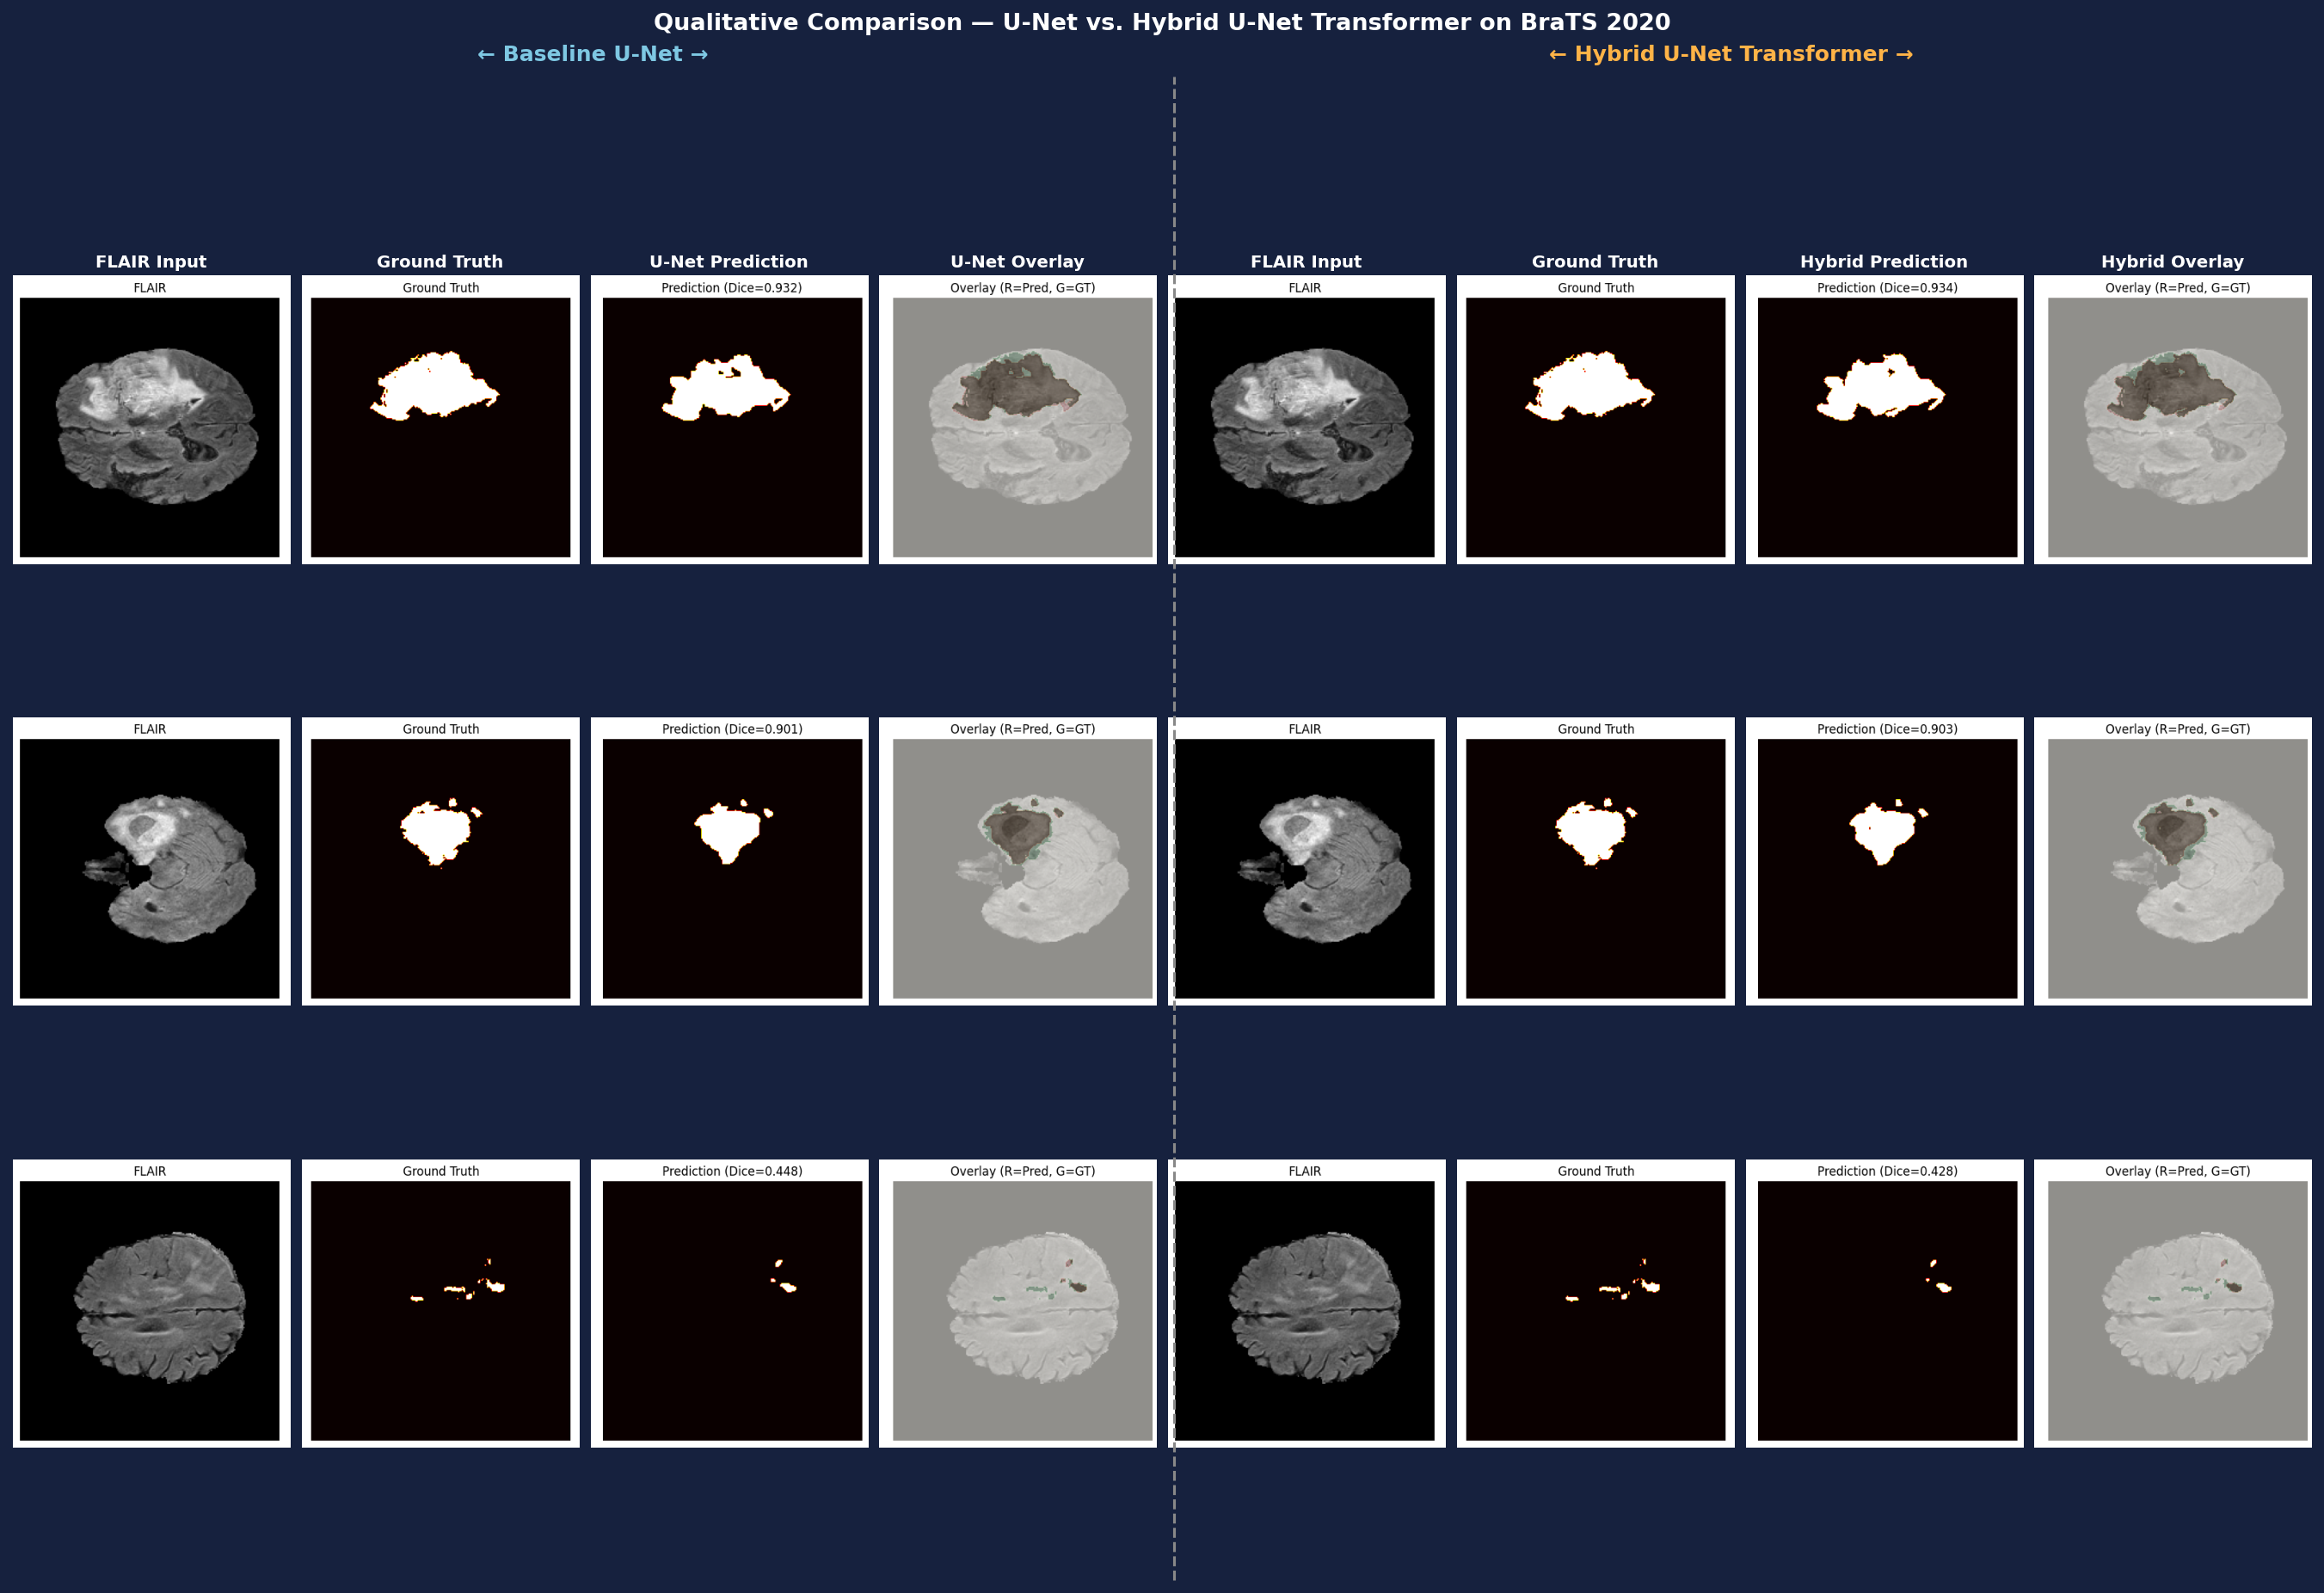
\includegraphics[width=\textwidth]{fig4_qualitative.png}
    \caption{Visual comparison of three validation cases. Left half: Baseline U-Net predictions. Right half: Hybrid U-Net Transformer predictions. Each group shows: FLAIR input, ground truth mask, model prediction, and overlay. The Hybrid model produces smoother boundaries and fewer false positive regions.}
\end{figure}

% ─────────────────────────────────────────────────────────────────────────────
\section{Discussion}
% ─────────────────────────────────────────────────────────────────────────────

\subsection{Why Does the Transformer Help?}

Convolutional layers look at only a small local area (e.g., 3$\times$3 pixels) at a time. To understand the full tumor extent, information must travel through many layers. The Transformer connects all 196 spatial positions (14$\times$14 grid) directly in every block, so it can immediately relate different parts of the image.

This global reasoning is especially useful when:
\begin{itemize}
    \item Tumors are large and spread across much of the image (FLAIR edema)
    \item Tumor shapes are irregular or concave
    \item There are multiple disconnected tumor regions
\end{itemize}

\subsection{Why Does Standard Deviation Decrease?}

The reduction in Dice standard deviation from 0.1993 to 0.1853 is as important as the mean improvement. It means the Hybrid model produces fewer completely wrong predictions on difficult slices. In clinical use, a model that is consistent and reliable on all cases is more valuable than one that is excellent on easy cases but fails on hard ones.

\subsection{Limitations}

\begin{table}[H]
    \centering
    \caption{Current limitations and planned future work}
    \begin{tabular}{ll}
        \toprule
        \textbf{Limitation} & \textbf{Planned Solution} \\
        \midrule
        2D slices — no 3D context & Use 3D model on larger GPU \\
        Binary segmentation only & Extend to 3-class (edema, core, enhancing) \\
        Training from scratch & Use pre-trained Transformer weights \\
        Boundary loss not used & Activate with weight 0.1--0.2 \\
        Only BraTS 2020 tested & Test on BraTS 2021 and clinical data \\
        \bottomrule
    \end{tabular}
\end{table}

% ─────────────────────────────────────────────────────────────────────────────
\section{Conclusion}
% ─────────────────────────────────────────────────────────────────────────────

This project implemented and evaluated a Hybrid U-Net Transformer for brain tumor segmentation on MRI. The key results are:

\begin{itemize}
    \item The Hybrid model achieves \textbf{Dice = 0.8409} vs.\ 0.8339 for the U-Net baseline (+0.70\%)
    \item \textbf{IoU improves} from 0.7512 to 0.7577 (+0.66\%)
    \item \textbf{Hausdorff Distance decreases} from 14.984 to 14.266 pixels (better boundary accuracy)
    \item \textbf{Standard deviation drops} from 0.1993 to 0.1853 (more consistent predictions)
    \item The entire system runs on a \textbf{consumer GPU} (RTX 4060, 8 GB) in 3--4 hours
\end{itemize}

Adding a small Transformer module to the U-Net bottleneck provides meaningful improvements in segmentation quality with only a modest increase in parameters (7.8M $\to$ 12.4M) and training time. This demonstrates that global self-attention is beneficial even for 2D medical image segmentation without any pre-training.

% ─────────────────────────────────────────────────────────────────────────────
\section*{References}
% ─────────────────────────────────────────────────────────────────────────────
\addcontentsline{toc}{section}{References}

\begin{enumerate}[label={[\arabic*]}]
    \item Ronneberger O., Fischer P., Brox T. \textit{U-Net: Convolutional Networks for Biomedical Image Segmentation.} MICCAI, 2015.
    \item Dosovitskiy A. et al. \textit{An Image is Worth 16×16 Words: Transformers for Image Recognition at Scale.} ICLR, 2021.
    \item Chen J. et al. \textit{TransUNet: Transformers Make Strong Encoders for Medical Image Segmentation.} arXiv:2102.04306, 2021.
    \item Menze B. H. et al. \textit{The Multimodal Brain Tumor Image Segmentation Benchmark (BRATS).} IEEE Trans.\ Med.\ Imaging, 2015.
    \item Bakas S. et al. \textit{Advancing the Cancer Genome Atlas Glioma MRI Collections.} Scientific Data, 2017.
    \item Isensee F. et al. \textit{nnU-Net: A Self-Configuring Method for Deep Learning-Based Biomedical Image Segmentation.} Nature Methods, 2021.
    \item Milletari F., Navab N., Ahmadi S. \textit{V-Net: Fully Convolutional Neural Networks for Volumetric Medical Image Segmentation.} 3DV, 2016.
    \item Lin T.-Y. et al. \textit{Focal Loss for Dense Object Detection.} ICCV, 2017.
    \item Kervadec H. et al. \textit{Boundary Loss for Highly Unbalanced Segmentation.} MIDL, 2019.
    \item Buslaev A. et al. \textit{Albumentations: Fast and Flexible Image Augmentations.} Information, 2020.
\end{enumerate}

\end{document}
